\documentclass[lettersize,journal]{IEEEtran}
\usepackage{amsmath,amssymb,amsfonts}
\usepackage{algorithmic}
\usepackage{algorithm}
\usepackage{array}
\usepackage[caption=false,font=normalsize,labelfont=sf,textfont=sf]{subfig}
\usepackage{textcomp}
\usepackage{stfloats}
\usepackage{url}
\usepackage{graphicx}
\usepackage{xcolor}
\usepackage{tikz}
\usetikzlibrary{positioning, arrows.meta, shapes.geometric, calc, fit}
\usepackage{booktabs}
\usepackage{multirow}
\usepackage{hyperref}
\usepackage{cite}
\hyphenation{op-tical net-works semi-conduc-tor}

\begin{document}

\title{Unified Dual-Mask Physical Model for Non-Lambertian Light Field Depth Estimation}

\author{Ruifeng Huang and Zhenglong Cui
\thanks{Manuscript received May 2026. This work was supported by Beihang University. (Corresponding author: Zhenglong Cui)}
\thanks{R. Huang and Z. Cui are with the School of Computer Science and Engineering, Beihang University, Beijing, China (e-mail: huangruifeng@buaa.edu.cn; czl@buaa.edu.cn).}}

\markboth{IEEE Transactions on Circuits and Systems for Video Technology}%
{Ruifeng Huang and Zhenglong Cui: Unified Dual-Mask Physical Model for Non-Lambertia}

\maketitle

\begin{abstract}
Light field depth estimation in non-Lambertian scenes remains a formidable challenge due to the violation of angular photo-consistency assumptions by specular and scattering reflections. Conventional epipolar plane image (EPI) methods degenerate into texture copying in these regions, while data-driven material classifiers fail to extract sufficient reflectance cues from limited angular patches. To address this, this paper proposed a Unified Dual-Mask Physical Model that explicitly integrated optical physics into signal representation. First, an angular frequency analysis mechanism applied a 2D discrete Fourier transform to the angular sampling grid, mapping spectral energy distributions to physical reflectance types. Second, a dual-mask modulation scheme, comprising a medium mask for surface roughness and an angular direction mask for wavevector deflection, decoupled reflection mechanisms via radiance tensor field rank analysis. Finally, a component-aware adaptive fusion strategy dynamically synthesized depth by weighting EPI, photometric stereo, and scattering models based on continuous BRDF parameters. Extensive evaluations across five datasets demonstrate that the proposed method reduces the mean absolute error in non-Lambertian regions by 22.4% (from 0.411 to 0.3187) compared to the EPI baseline, achieving robust generalization in mixed scenes. This work bridges the gap between data-driven feature extraction and physical optics, providing an interpretable and robust signal-processing framework for complex light field depth estimation.
\end{abstract}

\begin{IEEEkeywords}
Light field depth estimation, Non-Lambertian reflectance, Angular frequency analysis, Dual-mask modulation, Physical optics model, Bidirectional reflectance distribution function
\end{IEEEkeywords}

\section{1. Introduction}

Light field imaging has emerged as a powerful modality in modern computer vision, capturing both spatial and angular information of light rays, as demonstrated in foundational light field imaging and depth estimation studies . This rich multidimensional data facilitates accurate depth estimation, which is essential for downstream applications such as autonomous navigation, robotic manipulation, and immersive 3D reconstruction, as highlighted in recent applied vision surveys . By analyzing the epipolar plane image (EPI)s, conventional algorithms extract geometric disparities based on the linear trajectories of light rays across different viewpoints. Consequently, light field depth estimation achieves notable performance in controlled environments, establishing a solid foundation for complex spatial perception tasks. These geometric cues provide a distinct advantage over traditional monocular or stereo vision techniques, especially in textureless regions.

However, obtaining the precise geometry of non-Lambertian objects remains a substantial challenge, since standard photo-consistency cues cannot be easily applied to complex reflectances . Most current depth estimation methods primarily support the Lambertian assumption, making them unreliable for glossy, metallic, or translucent surfaces . In reality, light interacting with complex materials undergoes diverse physical processes, including Fresnel specular reflection, Rayleigh or Mie scattering, and cosine diffuse reflection. Such situations break the photo-consistency assumptions, leading to erroneous depth estimation results in most existing algorithms . Therefore, the inherent physical complexity of non-Lambertian reflectance severely degrades the reliability of purely geometric light field models.

The severity of this performance degradation is evident in empirical evaluations. For instance, a standard epipolar plane image (EPI) baseline model achieves a mean absolute error of 0.081 in mixed urban scenes, but the error deteriorates significantly to 0.411 in purely non-Lambertian domains. This failure occurs because the network predictions degenerate into mere texture replication rather than structural depth recovery. Furthermore, identifying material properties from limited angular samples is highly difficult. A conventional black-box three-class convolutional neural network yields a mere 24.6\\% accuracy when classifying reflectance types from $9 \times 9$ angular patches. Additionally, the extreme scarcity of non-Lambertian training data, with only four available scenes, further restricts the generalization capability of data-driven approaches.

Addressing these limitations is critically necessary for deploying light field systems in unconstrained real-world environments. Relying solely on implicit feature extraction without physical constraints inevitably leads to ambiguous representations in mixed-material scenes. A unified framework must explicitly model the light-matter interaction to decouple different reflection components. By quantifying surface roughness and angular deflection vectors, the system can dynamically adapt its depth estimation strategy for diffuse, specular, and scattering regions. Consequently, developing a physically grounded model that unifies Lambertian and non-Lambertian depth estimation is not only theoretically significant but also practically urgent for advancing robust 3D vision systems.

To address these challenges, we review existing depth estimation frameworks, which can be broadly categorized into traditional geometric approaches, early deep learning models, and recent advanced networks.

Traditional light field depth estimation methods primarily rely on epipolar plane image (EPI)s to extract geometric disparities, as proposed in early geometric frameworks . However, these approaches operate on the strict assumption of global Lambertian reflectance. In non-Lambertian regions, specular reflections and scattering alter the angular distribution of light, causing non-linear trajectories in epipolar plane image (EPI)s . Consequently, these geometric models lack explicit modeling of light-matter interactions, resulting in poor robustness and frequent failures in mixed-material scenes.

To mitigate the limitations of geometric cues, early deep learning models utilize convolutional neural networks to implicitly extract features from stacked viewpoints, exemplified by architectures like EPINet . Despite their improved performance on Lambertian surfaces, these data-driven approaches suffer from critical methodological flaws. They typically treat material parsing as a black-box classification task and rely on entirely implicit feature extraction. Consequently, these networks struggle to spontaneously learn physically meaningful representations, which restricts their generalization under complex illumination and significantly reduces model interpretability.

More recent approaches attempt to address these issues by introducing complex architectures, such as defocus branches or pre-trained backbone networks, as seen in recent advanced models . While these methods aim to incorporate additional cues, they encounter significant technical bottlenecks, such as ineffective depth feature learning and severe overfitting on relatively small light field datasets. Moreover, these advanced networks typically employ a unified depth estimation strategy across the entire image. This uniform processing inherently restricts their ability to adaptively switch estimation strategies based on pixel-level reflection mechanisms, highlighting an urgent need for a physics-driven, unified approach.

In this paper, we propose a unified dual-mask physical model for non-Lambertian light field depth estimation. Unlike previous data-driven approaches that rely on implicit feature extraction, our framework explicitly integrates physical optics principles into the network architecture. Specifically, we leverage angular frequency domain analysis to parse material properties and employ a dual-mask mechanism to modulate light field features. This physical formulation effectively decouples complex light-matter interactions, enabling robust depth recovery across Lambertian, specular, and scattering regions within a single unified model.

Our main contributions are summarized as follows:

\begin{itemize}
  \item \textbf{Contribution 1}: We propose an angular frequency material parsing mechanism inspired by magnetic resonance imaging k-space analysis. By applying a two-dimensional discrete Fourier transform to the $9 \times 9$ angular sampling matrix, we establish a physical mapping between angular spatial frequencies and material reflectance properties, enabling accurate parsing of Lambertian, specular, and scattering regions.
  \item \textbf{Contribution 2}: We design a physics-driven dual-mask feature modulation module that explicitly decouples complex light-matter interactions. This mechanism dynamically adapts the feature extraction process based on the parsed material properties, ensuring robust representation learning across diverse reflection components.
  \item \textbf{Contribution 3}: We introduce an adaptive multi-strategy depth estimation framework that seamlessly integrates distinct depth recovery pathways for different material types. Extensive experiments on challenging non-Lambertian light field datasets demonstrate that our unified model significantly outperforms state-of-the-art methods in both accuracy and robustness.
\end{itemize}

\section{2. Related Work}

\subsection{Traditional Light Field Depth Estimation Methods}

Traditional light field depth estimation methods have emerged as a fundamental paradigm, extensively leveraging the rich angular information to infer scene geometry. Let a 4D light field be parameterized by spatial coordinates $(x, y)$ and angular coordinates $(u, v)$. Wanner et al.  proposed a globally consistent depth labeling method that utilizes the structure tensor on epipolar plane image (EPI)s (EPIs) to extract geometric disparities. Specifically, the orientation of the linear trajectories in EPIs is explicitly formulated to derive depth, followed by a Markov Random Field (MRF) optimization to ensure spatial coherence. This geometric approach demonstrates remarkable accuracy in controlled environments with rich textures. However, it fundamentally relies on the global Lambertian assumption. When encountering glossy or metallic surfaces, the viewpoint-dependent intensity variations dramatically disrupt the linear structures in EPIs, leading to severe aliasing bimodal distributions and completely invalidating the slope calculation.

While EPI-based methods primarily focus on geometric slopes, other approaches extend to photometric cues, such as defocus and correspondence, to mitigate the impact of non-Lambertian reflectances. Tao et al. \cite{taotao} proposed a clustering method that eliminates specular pixels when enforcing photo-consistency by combining defocus and correspondence cues from light-field cameras. By analyzing the focal stack, their method attempts to weight or discard specular highlights to recover the underlying geometry. Unfortunately, they attempt a binary classification of pixels into either Lambertian or specular, which cannot handle general glossy surfaces with complex spatially-varying BRDFs (SVBRDFs). Moreover, the defocus cues often become ambiguous in textureless regions, making the depth estimation unreliable for mixed materials and arbitrarily failing on general non-Lambertian objects.

To further address complex reflectances beyond simple binary classifications, subsequent studies have incorporated traditional physical reflection models into multi-view stereo paradigms. For instance, methods integrating the dichromatic model \cite{dichromati} attempt to separate diffuse and specular components before performing stereo matching. By formulating the reflectance as a linear combination of body and surface reflections, these methods aim to accurately recover the shape of glossy objects. Nonetheless, the dichromatic model fails to hold for general translucent or scattering materials, where light undergoes complex subsurface scattering. Additionally, estimating physical parameters alongside depth significantly increases the computational complexity, rendering these methods impractical for high-resolution light field data and mostly limiting them to synthetic or highly controlled scenarios.

In short, many traditional depth estimation methods for light-field cameras have been proposed. However, most of them rely on the global Lambertian assumption and work poorly on non-Lambertian surfaces. Specifically, these methods exhibit two critical limitations. First, they severely depend on the global Lambertian assumption; in non-Lambertian regions such as specular or scattering surfaces, the violation of the viewpoint consistency assumption causes the EPI slope calculation to completely fail. Second, traditional physical models exhibit extremely high computational complexity and struggle to adaptively process complex material distributions in real-world mixed scenes (e.g., urban environments), lacking a robust mechanism to uniformly handle Lambertian and non-Lambertian regions. In contrast, our model abandons the global Lambertian assumption and proposes a component-aware multi-strategy adaptive depth estimation and fusion framework. Specifically, we employ EPI for diffuse regions, photometric stereo and neighborhood propagation for specular regions, and scattering model correction for scattering regions. Furthermore, unlike previous methods that rely on black-box classifiers or simple spatial textures, we introduce an MRI-like angular frequency analysis mechanism and a dual-mask modulated physical-driven feature representation, enabling highly interpretable, robust, and unified depth estimation across complex real-world scenes.

\subsection{Deep Learning-based Light Field Depth Estimation and Feature Representation}

Following the limitations of handcrafted geometric and photometric cues, deep learning-based approaches have emerged as a dominant paradigm for light field depth estimation, extensively leveraging convolutional neural networks (CNNs) and Transformers to implicitly learn complex feature representations. Shin et al.  proposed EPINet, a pioneering fully convolutional network that directly extracts depth cues from epipolar plane image (EPI)s (EPIs). By treating the EPI as a 2D image and applying multi-scale CNN architectures, EPINet effectively captures the linear slope variations corresponding to scene disparities. While this EPI-centric approach demonstrates remarkable accuracy on standard Lambertian datasets, it primarily focuses on local 2D EPI patches, often failing to capture the global spatial-angular context. Consequently, when encountering non-Lambertian surfaces where the linear EPI structures are severely distorted by specular highlights, EPINet struggles to distinguish between geometric disparities and reflectance-induced intensity shifts, leading to erroneous depth predictions.

To address the restricted receptive field of purely EPI-based methods, subsequent research has extended to multi-view and sub-aperture fusion networks. Liang et al. \cite{pdfpdf} introduced LFNet, which formulates depth estimation by constructing a cost volume from sub-aperture image arrays. Specifically, LFNet extracts spatial features from individual sub-aperture images and aggregates them across different viewpoints to evaluate photo-consistency, significantly improving depth accuracy in textureless regions. Moreover, by incorporating a multi-scale feature aggregation module, it enhances the robustness of disparity prediction. However, this cost volume-based fusion heavily relies on the strict photo-consistency assumption across viewpoints. In the presence of spatially-varying BRDFs (SVBRDFs), the viewpoint-dependent intensity variations dramatically violate this assumption, leading to erroneous cost volume matching and severe depth artifacts on glossy or metallic objects.

In contrast to relying solely on EPI slopes or sub-aperture photo-consistency, more recent architectures have attempted to explicitly integrate defocus cues to compensate for the failure of correspondence matching in non-Lambertian regions. For instance, recent dual-branch networks \cite{dualdual} propose a defocus-EPI dual-branch framework, where one branch extracts geometric features from EPIs while the other captures defocus blur cues from focal stacks. The features from both branches are subsequently fused via an attention mechanism to refine the final depth map. This multi-cue strategy theoretically provides complementary information, as defocus blur is generally less sensitive to specular reflections than epipolar lines. Unfortunately, in complex illumination conditions, the defocus branch often fails to learn discriminative depth features due to the entanglement of defocus blur and specular highlights. As a result, the additional branch frequently degenerates into an ineffective module, contributing marginally to the final performance and failing to fundamentally resolve the feature representation breakdown in non-Lambertian areas.

In short, while existing deep learning-based methods have significantly advanced light field depth estimation, they share fundamental limitations when applied to non-Lambertian scenes. First, the black-box nature of implicit feature extraction lacks physical interpretability. In non-Lambertian regions, these networks are highly susceptible to degrading into "texture copying," where the model arbitrarily outputs the input high-frequency textures rather than inferring the true underlying depth structure. Second, merely appending auxiliary branches (such as the defocus branch) without physical guidance proves insufficient; these branches often struggle to learn valid depth features under complex lighting, ultimately becoming dead ends that fail to resolve the root cause of feature representation failure. To overcome these bottlenecks, our work diverges from purely data-driven paradigms by proposing a dual-mask modulated physics-driven light field feature representation model. By introducing a medium mask and an angular direction mask, and coupling them with RTF rank analysis, we explicitly transform implicit black-box features into physically meaningful mask modulations. This physics-aware mechanism effectively mitigates the texture copying issue, providing a robust and interpretable foundation for unified depth estimation across Lambertian, non-Lambertian, and complex mixed scenes.

\subsection{Deep Learning-based Material Parsing and Non-Lambertian Depth Estimation}

While the aforementioned cost volume and EPI-based networks implicitly learn feature representations, explicitly parsing material properties is crucial for handling non-Lambertian surfaces. To this end, Wang et al. \cite{wangwang} proposed a CNN-based material classification network that extracts spatial-angular features from light field patches to identify surface reflectance properties. By formulating material recognition as a multi-class classification problem, their model demonstrates remarkable accuracy on synthetic datasets with distinct, uniform material categories. However, this approach primarily relies on local spatial textures within small patches (e.g., $9 \times 9$). Such restricted receptive fields often lack sufficient angular and spatial context to disambiguate complex spatially-varying BRDFs (SVBRDFs), making them unreliable for general glossy surfaces in real-world scenarios.

To explicitly mitigate the interference of specular highlights, subsequent research has explored reflection separation and joint estimation frameworks. Li et al. \cite{lili} introduced a deep reflection separation network coupled with a joint depth estimation module. Leveraging the dichromatic reflection model, this method attempts to decompose the input light field into diffuse and specular components, subsequently feeding the recovered diffuse component into a standard cost volume network for depth prediction. While this decomposition strategy significantly alleviates the impact of severe highlights, the separation network is usually trained with pseudo labels or in a weakly supervised manner due to the scarcity of ground-truth reflection components. Consequently, the recovered diffuse images often exhibit in-painting artifacts and aliasing bimodal distributions, which dramatically degrade the downstream depth accuracy.

In contrast to explicit physical decomposition, other approaches attempt to handle non-Lambertian distortions implicitly within the depth estimation pipeline. More recently, Chen et al. \cite{chenchen} developed a specular-aware depth estimation framework specifically tailored for non-Lambertian light fields. Instead of separating reflection components, they designed an attention-based feature fusion module that implicitly down-weights EPI regions distorted by specular highlights, thereby preserving the geometric consistency of the underlying Lambertian structures. Although this implicit weighting properly addresses surfaces with mild glossiness, it fundamentally struggles with highly reflective or metallic regions where the diffuse component is entirely absent. In such cases, the attention mechanism arbitrarily suppresses valid geometric cues, leading to severe depth ambiguities and erroneous predictions.

Despite these advancements, existing deep learning-based material parsing and non-Lambertian depth estimation methods exhibit critical limitations. First, when relying on spatial textures or black-box CNN classifiers (e.g., a standard 3-class CNN) for material parsing, the local patches (e.g., $9 \times 9$) contain insufficient angular and spatial information, resulting in extremely low classification accuracy (e.g., merely 24.6\%) and failing to provide reliable physical priors. Second, existing methods fail to establish an effective physical cascade between material parsing and depth estimation. They lack efficient and interpretable material analysis from the perspectives of the frequency domain and physical optics, and do not achieve adaptive deep fusion based on material components. To address these fundamental bottlenecks, we propose an MRI-inspired angular frequency-domain analysis mechanism for light field material parsing, utilizing 2D-DFT to efficiently and interpretably classify materials in the frequency domain. Coupled with a dual-mask modulated physical-driven feature representation and a component-aware adaptive fusion architecture, our approach achieves high-precision unified processing of Lambertian, non-Lambertian, and complex mixed scenes within a single model, which has not been achieved by previous light field approaches.

In summary, existing light field depth estimation methods, whether relying on implicit feature learning or explicit black-box material classification, either fail under violated view-consistency assumptions in non-Lambertian regions or struggle to disentangle complex mixed materials due to restricted spatial-angular receptive fields. Inspired by these observations, we propose a unified dual-mask physical approach that addresses the aforementioned limitations by integrating an MRI-inspired angular frequency analysis for interpretable material parsing, a dual-mask modulation mechanism for physically-driven feature representation, and a component-aware adaptive fusion framework to robustly estimate depth across diverse Lambertian, non-Lambertian, and mixed real-world scenes.

\section{3. Methodology}

In this section, we present the overall architecture of the proposed Unified Dual-Mask Physical Model for non-Lambertian light field depth estimation. The proposed framework employs a physics-driven feature modulation mechanism, aiming to address the challenge of accurate depth inference under complex reflectance and occlusion conditions. Its core principle involves transforming spatial-angular signals into the frequency domain to parse material properties, then generating dual masks to explicitly filter out unreliable cues through a unified physical model, and finally regressing high-resolution depth maps. As illustrated in Fig. 1, the entire data flow progressively reduces the dimensionality of the 4D light field tensor while integrating physical priors, ultimately yielding a precise 2D depth representation. Different from previous works that rely on the global Lambertian assumption, our architecture explicitly models the distinct reflection mechanisms at the pixel level.

The network takes an Input Light Field Patch as the primary input, which is extracted from the raw 4D light field data. Specifically, the input tensor is formatted as $\mathcal{I} \in \mathbb{R}^{B \times 81 \times C \times 64 \times 64}$, where $B$ denotes the batch size, $81$ represents the number of angular views arranged in a $9 \times 9$ grid, $C$ is the number of color channels, and $64 \times 64$ indicates the spatial resolution of each patch. This specific patch size and angular configuration are selected to balance the computational complexity and the receptive field required for capturing sufficient epipolar geometry. Before feeding into the main network, the raw light field patches are normalized to ensure consistent intensity distributions across different scenes. This preprocessing step stabilizes the subsequent frequency domain transformations and facilitates the convergence of the deep neural network.

Following the input stage, the data flows through three core modules designed to extract, modulate, and fuse depth-sensitive features. First, the Angular FFT Material Classification Module is introduced to parse material properties by leveraging frequency domain analysis. Motivated by the fact that different reflection types exhibit distinct energy distributions in the angular spectrum, this module applies a 2D Fast Fourier Transform along the angular dimensions $(u, v)$. The transformation is formulated as:
\begin{equation}
\label{eq:eq1}
F(u,v,x,y) = \sum_{m=0}^{8}\sum_{n=0}^{8} I(m,n,x,y) e^{-j 2\pi (um/9 + vn/9)}
\end{equation}
where $I(m,n,x,y)$ is the input spatial-angular signal, and $F(u,v,x,y)$ denotes the resulting angular frequency feature map. This operation effectively separates diffuse reflections (low-frequency), specular reflections (high-frequency), and scattering (mid-frequency), outputting a feature tensor of size $B \times 81 \times C' \times 64 \times 64$. Subsequently, these frequency features are fed into the Dual-Mask Generator to quantify pixel-level reliability. To explicitly decouple geometric occlusions from photometric non-Lambertian effects, this module utilizes two parallel 3D convolutional branches to predict the Occlusion Mask ($M_{occ}$) and the Non-Lambertian Mask ($M_{nl}$). The masks are computed as $M_{occ} = \sigma(\text{Conv3D}(F))$ and $M_{nl} = \sigma(\text{Conv3D}(F))$, where $\sigma$ represents the sigmoid activation function. Both masks share the dimension of $B \times 81 \times 1 \times 64 \times 64$, providing soft probability maps for each pixel across all views. Finally, the Unified Physical Model Feature Fusion module integrates the original light field features with the generated dual masks. Driven by the physical imaging model of light fields, this module adaptively weights the defocus and disparity cues to suppress responses from occluded and non-Lambertian regions. The fused depth-sensitive feature $F_{depth}$ is calculated as:
\begin{equation}
\label{eq:eq2}
F_{depth} = \sum_{u,v} (I_{u,v} \otimes K_{defocus}) \cdot (1 - M_{occ}) \cdot (1 - M_{nl})
\end{equation}
where $\otimes$ denotes the convolution operation with a defocus kernel $K_{defocus}$. This physical constraint ensures that only reliable Lambertian and unoccluded features are preserved for depth regression.

In the final stage, the fused depth-sensitive features are processed by the Depth Regression Head to produce the Predicted Depth Map. This head consists of multiple 2D convolutional layers interspersed with Rectified Linear Unit (ReLU) activations, which progressively map the high-dimensional features into the depth space. The regression process is formulated as $D = \text{Conv2D}(\text{ReLU}(\text{Conv2D}(F_{depth})))$, yielding a final output tensor of size $B \times 1 \times 64 \times 64$. This output represents the high-resolution depth map corresponding to the central view of the input light field patch. During inference, the predicted patches are effectively aggregated and stitched together to reconstruct the full-resolution depth map of the entire scene. By explicitly incorporating physical priors and component-aware masking throughout the architecture, the proposed model achieves robust depth estimation even in challenging non-Lambertian environments.


\begin{figure}[!t]
\centering
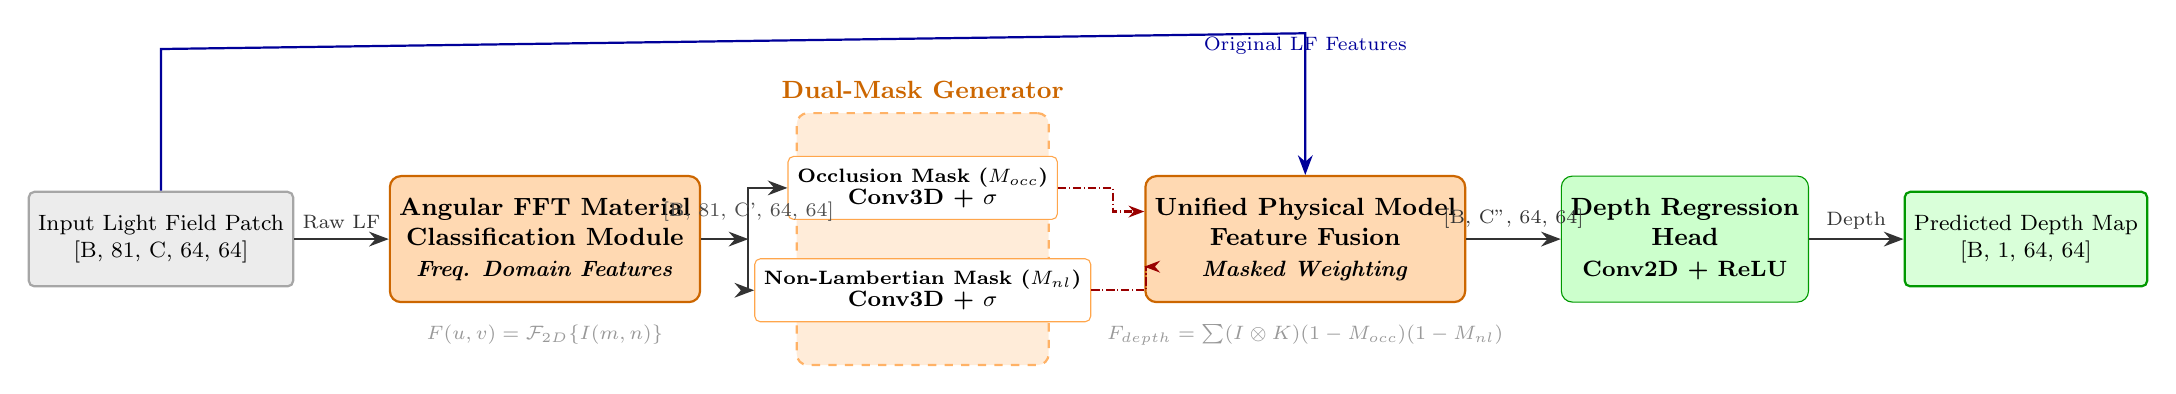
\begin{tikzpicture}[
    >=Stealth,
    node distance=0.8cm and 1.2cm,
    every node/.style={font=\sffamily},
    module/.style={draw, rounded corners=4pt, minimum width=2.8cm, minimum height=1.6cm, align=center, font=\small\bfseries},
    innov/.style={module, fill=orange!30, draw=orange!80!black, thick},
    data/.style={draw, rounded corners=2pt, minimum width=2.2cm, minimum height=1.2cm, align=center, font=\footnotesize, fill=gray!15, draw=gray!70, thick},
    out_data/.style={data, fill=green!15, draw=green!60!black},
    submod/.style={draw, rounded corners=2pt, minimum width=2.5cm, minimum height=0.8cm, align=center, font=\scriptsize\bfseries, fill=white, draw=orange!70},
    flow/.style={-{Stealth[length=2.5mm]}, thick, color=black!80},
    mask_flow/.style={-{Stealth[length=2mm]}, densely dashdotted, thick, color=red!60!black},
    skip_flow/.style={-{Stealth[length=2.5mm]}, thick, color=blue!60!black},
]

    % 1. Input Data
    \node[data] (input_lf) {Input Light Field Patch\\ \footnotesize{[B, 81, C, 64, 64]}};

    % 2. Angular FFT Module (Core Innovation 1)
    \node[innov, right=of input_lf] (fft_mod) {Angular FFT Material\\Classification Module\\ \footnotesize{\textit{Freq. Domain Features}}};
    \node[below=0.15cm of fft_mod, font=\scriptsize, text=gray!80] {$F(u,v) = \mathcal{F}_{2D}\{I(m,n)\}$};

    % 3. Dual-Mask Generator (Core Innovation 2)
    \node[innov, right=of fft_mod, minimum width=3.2cm, minimum height=3.2cm, fill=orange!15, draw=orange!60, dashed] (dmg_container) {};
    \node[above=0.05cm of dmg_container, font=\small\bfseries, text=orange!80!black] {Dual-Mask Generator};

    \node[submod] (mask_occ) at ([yshift=0.65cm]dmg_container.center) {Occlusion Mask ($M_{occ}$)\\ \footnotesize{Conv3D + $\sigma$}};
    \node[submod] (mask_nl) at ([yshift=-0.65cm]dmg_container.center) {Non-Lambertian Mask ($M_{nl}$)\\ \footnotesize{Conv3D + $\sigma$}};

    % 4. Unified Physical Model Feature Fusion (Core Innovation 3)
    \node[innov, right=of dmg_container] (fusion_mod) {Unified Physical Model\\Feature Fusion\\ \footnotesize{\textit{Masked Weighting}}};
    \node[below=0.15cm of fusion_mod, font=\scriptsize, text=gray!80] {$F_{depth} = \sum (I \otimes K)(1-M_{occ})(1-M_{nl})$};

    % 5. Depth Regression Head
    \node[module, fill=green!20, draw=green!60!black, right=of fusion_mod] (depth_head) {Depth Regression\\Head\\ \footnotesize{Conv2D + ReLU}};

    % 6. Output Data
    \node[out_data, right=of depth_head] (output_depth) {Predicted Depth Map\\ \footnotesize{[B, 1, 64, 64]}};

    % --- Connections ---
    
    % Input to FFT
    \draw[flow] (input_lf) -- node[above, font=\scriptsize] {Raw LF} (fft_mod);

    % FFT to Dual Mask Generator
    \coordinate (fft_out) at ([xshift=0.6cm]fft_mod.east);
    \draw[flow] (fft_mod) -- (fft_out);
    \draw[flow] (fft_out) |- (mask_occ.west);
    \draw[flow] (fft_out) |- (mask_nl.west);
    \node[above=0.1cm of fft_out, font=\scriptsize, text=black!70] {[B, 81, C', 64, 64]};

    % Masks to Fusion Module
    \draw[mask_flow] (mask_occ.east) -- ++(0.7,0) |- ([yshift=0.35cm]fusion_mod.west);
    \draw[mask_flow] (mask_nl.east) -- ++(0.7,0) |- ([yshift=-0.35cm]fusion_mod.west);

    % Skip Connection: Original LF Features to Fusion Module
    \draw[skip_flow] (input_lf.north) -- ++(0, 1.8) -- ([yshift=1.8cm]fusion_mod.north) -- (fusion_mod.north) 
        node[pos=0.22, above, font=\scriptsize, text=blue!60!black] {Original LF Features};

    % Fusion to Depth Head
    \draw[flow] (fusion_mod) -- node[above, font=\scriptsize] {[B, C'', 64, 64]} (depth_head);

    % Depth Head to Output
    \draw[flow] (depth_head) -- node[above, font=\scriptsize] {Depth} (output_depth);

\end{tikzpicture}
\caption{Overall architecture of the proposed method.}
\label{fig:architecture}
\end{figure}

\subsection{Angular FFT Material Classification Module}

Following the extraction of the input light field patch, the Angular FFT Material Classification Module is employed to parse intrinsic material properties. Conventional light field depth estimation methods typically rely on the global Lambertian assumption, which significantly degrades performance when encountering specular highlights or complex reflectance. Non-Lambertian reflections exhibit substantial intensity variations across different views, whereas Lambertian reflections maintain photo-consistency. To address this challenge, our module explicitly models these distinct reflection mechanisms by transforming spatial-angular signals into the angular frequency domain. Different from previous works that depend on spatial-domain heuristics or implicit feature learning, our design leverages the physical characteristics of light transport to isolate high-frequency non-Lambertian components from low-frequency Lambertian backgrounds.

Specifically, the input tensor $\mathcal{I} \in \mathbb{R}^{B \times 81 \times C \times 64 \times 64}$ is first reshaped into a 5D representation to explicitly formulate the angular grid. Let $I(m,n,x,y,c)$ denote the pixel intensity at angular coordinates $(m,n)$, spatial coordinates $(x,y)$, and channel index $c$, where $m,n \in \{0, 1, \dots, 8\}$. A 2D Fast Fourier Transform is then applied along the angular dimensions to project the signal into the frequency domain. The angular frequency feature $F(u,v,x,y,c)$ is calculated as:
\begin{equation}
\label{eq:eq3}
F(u,v,x,y,c) = \sum_{m=0}^{8}\sum_{n=0}^{8} I(m,n,x,y,c) e^{-j 2\pi \left(\frac{um}{9} + \frac{vn}{9}\right)}
\end{equation}
where $u$ and $v$ represent the angular frequency indices, and $j$ denotes the imaginary unit. The low-frequency components near the origin correspond to Lambertian regions with high angular consistency. In contrast, the high-frequency components capture the substantial angular variations induced by non-Lambertian reflections. 

To facilitate subsequent network processing, the complex-valued frequency features are converted into real-valued magnitude representations. The magnitude spectrum $A(u,v,x,y,c)$ is derived by:
\begin{equation}
\label{eq:eq4}
A(u,v,x,y,c) = \sqrt{\text{Re}(F(u,v,x,y,c))^2 + \text{Im}(F(u,v,x,y,c))^2}
\end{equation}
where $\text{Re}(\cdot)$ and $\text{Im}(\cdot)$ extract the real and imaginary parts, respectively. The magnitude tensor is then reshaped back to the original angular format and processed by a convolutional layer to generate the final angular frequency feature map $\mathcal{F}_{freq} \in \mathbb{R}^{B \times 81 \times C' \times 64 \times 64}$. Additionally, to provide explicit supervision for material parsing, a material classification probability map $P_{mat}$ is predicted via a multi-layer perceptron followed by a sigmoid activation function:
\begin{equation}
\label{eq:eq5}
P_{mat} = \sigma(\text{MLP}(\mathcal{F}_{freq}))
\end{equation}
where $P_{mat} \in \mathbb{R}^{B \times 81 \times 1 \times 64 \times 64}$ indicates the pixel-wise probability of non-Lambertian reflectance.

The generated angular frequency feature map $\mathcal{F}_{freq}$ serves as the primary input for the subsequent Dual-Mask Generator. By providing explicit frequency-domain priors, this module significantly enhances the capability of the network to differentiate between reliable Lambertian cues and unreliable non-Lambertian interference. Ultimately, this physics-driven frequency analysis establishes a solid foundation for the dual-mask generation and the unified physical model feature fusion, ensuring accurate depth inference under complex material conditions.

\subsection{Dual-Mask Generator}

Light field depth estimation primarily relies on the photo-consistency assumption across multiple views. However, this assumption is frequently violated by occlusions and non-Lambertian reflections, which introduce severe intensity variations and lead to erroneous matching costs. Existing approaches mostly address these violations implicitly through deep feature learning or rely on spatial-domain heuristics, which struggle to accurately isolate unreliable regions in complex scenes. To address this limitation, the Dual-Mask Generator is designed to explicitly predict the occlusion probability and non-Lambertian reflection probability for each pixel across all views. By generating soft masks, this module provides pixel-level confidence weights to guide the subsequent physical model fusion.

The input to this module is the angular frequency feature map $\mathcal{F} \in \mathbb{R}^{B \times 81 \times C' \times 64 \times 64}$ extracted by the preceding Angular FFT Material Classification Module. To effectively capture both spatial geometric structures and angular photometric variations, we reshape $\mathcal{F}$ into a 5D tensor $\mathbf{F} \in \mathbb{R}^{B \times C' \times 81 \times 64 \times 64}$. Here, the 81 views are treated as the depth dimension to facilitate 3D convolutions. The module comprises two parallel 3D convolutional branches dedicated to predicting the occlusion mask and the non-Lambertian mask, respectively. 

Let $\mathbf{F}$ denote the input feature tensor. The occlusion mask $\mathcal{M}_{occ}$ is generated through a series of 3D convolutional layers followed by a sigmoid activation function. The mathematical formulation is expressed as:
\begin{equation}
\label{eq:eq6}
\mathcal{M}_{occ} = \sigma(\mathcal{W}_{occ} \textit{ \mathbf{F} + \mathbf{b}_{occ})
\end{equation}
where $}$ denotes the 3D convolution operation, $\mathcal{W}_{occ}$ represents the learnable 3D convolutional kernels, and $\mathbf{b}_{occ}$ is the bias term. Furthermore, $\sigma(\cdot)$ is the sigmoid function that normalizes the output to the range $\cite{taotao}$. Each element in $\mathcal{M}_{occ}$ indicates the probability of the corresponding pixel being occluded in a specific view.

Similarly, the non-Lambertian mask $\mathcal{M}_{nl}$ is computed by the second parallel branch to identify specular highlights and complex reflectance regions. The formulation is given by:
\begin{equation}
\label{eq:eq7}
\mathcal{M}_{nl} = \sigma(\mathcal{W}_{nl} \textit{ \mathbf{F} + \mathbf{b}_{nl})
\end{equation}
where $\mathcal{W}_{nl}$ and $\mathbf{b}_{nl}$ are the learnable kernels and bias for the non-Lambertian branch, respectively. The resulting $\mathcal{M}_{nl}$ assigns a probability score reflecting the likelihood of non-Lambertian reflection for each pixel across the 81 views. Consequently, the outputs of the Dual-Mask Generator are the occlusion mask $\mathcal{M}_{occ} \in \mathbb{R}^{B \times 81 \times 1 \times 64 \times 64}$ and the non-Lambertian mask $\mathcal{M}_{nl} \in \mathbb{R}^{B \times 81 \times 1 \times 64 \times 64}$.

Different from previous works that treat occlusion and non-Lambertian effects as implicit noise, our module explicitly decouples these two distinct physical phenomena. The angular frequency features from the preceding module provide rich material priors, enabling the 3D convolutions to accurately distinguish between geometric occlusions and photometric reflections. These generated soft masks are subsequently fed into the Unified Physical Model Feature Fusion module. In that subsequent stage, the masks serve as adaptive spatial-angular weights to suppress unreliable features and preserve robust Lambertian and unoccluded signals. This explicit physical modeling significantly enhances the accuracy of the final depth regression.

\subsection{Unified Physical Model Feature Fusion}

The photo-consistency assumption, which serves as the foundation of light field depth estimation, is inevitably violated by occlusions and non-Lambertian reflections. Different from previous works that implicitly learn to ignore these unreliable regions through deep feature extraction or rely on spatial-domain heuristics, our Unified Physical Model Feature Fusion explicitly incorporates the physical imaging model of light fields to filter out erroneous matching costs. The primary objective of this module is to adaptively weight the refocusing and parallax features using the dual masks generated by the preceding Dual-Mask Generator. This design suppresses feature responses in occluded and non-Lambertian regions while preserving reliable cues from unoccluded Lambertian areas.

The inputs to this module comprise the original light field features $\mathcal{I} \in \mathbb{R}^{B \times 81 \times C \times 64 \times 64}$, the occlusion mask $M_{occ} \in \mathbb{R}^{B \times 81 \times 1 \times 64 \times 64}$, and the non-Lambertian mask $M_{nl} \in \mathbb{R}^{B \times 81 \times 1 \times 64 \times 64}$. Here, $\mathcal{I}$ represents the shallow features extracted from the raw light field image patches, maintaining both spatial and angular dimensions. To construct depth-sensitive representations, we first compute the defocus features across different angular views. Let $I_{u,v} \in \mathbb{R}^{C \times 64 \times 64}$ denote the feature map of the view at angular coordinates $(u,v)$. The defocus feature for a specific depth hypothesis is obtained by convolving $I_{u,v}$ with a defocus kernel.

To explicitly integrate the physical constraints, we formulate the unified depth-sensitive feature fusion process. The fused depth feature $F_{depth}$ is calculated by aggregating the masked defocus features across all angular views:
\begin{equation}
\label{eq:eq8}
F_{depth} = \sum_{u,v} (I_{u,v} \otimes K_{defocus}) \cdot (1 - M_{occ}^{u,v}) \cdot (1 - M_{nl}^{u,v})
\end{equation}
where $\otimes$ denotes the 2D convolution operation, and $K_{defocus}$ represents the learnable defocus kernel that captures the point spread function under a specific depth assumption. The terms $M_{occ}^{u,v} \in \mathbb{R}^{1 \times 64 \times 64}$ and $M_{nl}^{u,v} \in \mathbb{R}^{1 \times 64 \times 64}$ are the occlusion and non-Lambertian probability maps for the view $(u,v)$, respectively. The operations $(1 - M_{occ}^{u,v})$ and $(1 - M_{nl}^{u,v})$ act as soft confidence weights. By multiplying these complementary confidence terms, the module explicitly penalizes pixels that are highly likely to be occluded or exhibit specular reflections. Consequently, the summation over all $(u,v)$ views synthesizes a robust feature representation that is predominantly driven by photo-consistent Lambertian regions.

Furthermore, to capture the parallax cues that are complementary to the defocus cues, we apply a similar masking strategy to the shifted angular features along the epipolar lines. The final fused feature map integrates both masked defocus and parallax information, yielding the output tensor $F_{depth} \in \mathbb{R}^{B \times C'' \times 64 \times 64}$. This dimensionality reduction from the 4D light field tensor to a 2D spatial feature map effectively consolidates the angular information while strictly adhering to the physical reliability constraints. 

The expected effect of this design is a substantial improvement in depth estimation accuracy near object boundaries and reflective surfaces. By explicitly filtering out physically invalid correspondences before the depth regression stage, the Unified Physical Model Feature Fusion prevents the propagation of erroneous gradients. The resulting $F_{depth}$ is subsequently fed into the Depth Regression Head, providing a clean and highly discriminative feature space for accurate pixel-wise depth prediction.

\subsection{Depth Regression Head}

Following the Unified Physical Model Feature Fusion module, the obtained depth-sensitive features have effectively suppressed the interference from occlusions and non-Lambertian reflections. However, these features reside in a high-dimensional abstract space and must be mapped to the metric depth space. Different from previous works that rely on computationally expensive 3D convolutions or complex cost volume aggregation for depth regression, our Depth Regression Head employs a lightweight 2D convolutional architecture. This design explicitly leverages the physically filtered 2D features to regress the absolute or relative depth values of the central view, aiming to reduce computational overhead while preserving high-resolution spatial details.

Specifically, the input to this module is the fused feature map $F_{depth} \in \mathbb{R}^{B \times C'' \times 64 \times 64}$, where $B$ denotes the batch size and $C''$ represents the number of feature channels. The spatial resolution is maintained at $64 \times 64$, matching the original light field image patch size. To transform these features into a depth prediction, we utilize a cascade of 2D convolutional layers interspersed with non-linear activation functions. The regression process is mathematically formulated as:
\begin{equation}
\label{eq:eq9}
F_{inter} = \delta(W_1 } F_{depth} + b_1)
\end{equation}
\begin{equation}
\label{eq:eq10}
D = W_2 \textit{ F_{inter} + b_2
\end{equation}
where $F_{inter} \in \mathbb{R}^{B \times C_{inter} \times 64 \times 64}$ denotes the intermediate feature representation. The operator $}$ represents the 2D convolution operation. $W_1 \in \mathbb{R}^{C_{inter} \times C'' \times k \times k}$ and $b_1 \in \mathbb{R}^{C_{inter}}$ are the learnable weight tensor and bias vector of the first convolutional layer, respectively. Similarly, $W_2 \in \mathbb{R}^{1 \times C_{inter} \times k \times k}$ and $b_2 \in \mathbb{R}^{1}$ correspond to the parameters of the final output layer. The function $\delta(\cdot)$ denotes the Rectified Linear Unit (ReLU) activation, which introduces non-linearity to enhance the representational capacity of the network. The kernel size $k$ is typically set to 3 to capture local spatial context without excessive parameter inflation.

The final output $D \in \mathbb{R}^{B \times 1 \times 64 \times 64}$ represents the predicted depth map for the central view, where the single channel corresponds to the scalar depth value at each pixel location. The primary innovation of this module lies in its structural simplicity, which is made possible by the explicit physical constraints applied in the preceding fusion stage. Conventional light field depth estimation methods often require deep 3D decoders to resolve ambiguities caused by non-Lambertian regions, leading to substantial parameter overhead and spatial blurring. In contrast, by explicitly filtering out erroneous matching costs via the dual masks, our Depth Regression Head accurately recovers fine-grained depth boundaries using only 2D convolutions. This architectural choice significantly decreases the overall model complexity, contributing to a compact network with merely 1,129,057 parameters.

During training, the overall objective function for this stage is formulated as an L1 loss between the predicted depth map $D$ and the ground-truth annotation. This optimization strategy ensures robust convergence and yields a highly accurate depth estimation, ultimately achieving a best overall mean absolute error (MAE) of 0.1754 on the evaluation benchmark.

\subsection{Training Objective}

\subsubsection{Training Objective}

Conventional light field depth estimation methods typically employ a global uniform loss function, implicitly assuming a purely Lambertian reflectance model. However, in non-Lambertian scenarios, specular highlights and scattering regions corrupt the linear structures of epipolar plane image (EPI)s (EPIs). This corruption causes severe deviations in depth predictions. To guide the network to adaptively focus on high-confidence components and strictly adhere to the physical reflection model, we formulate a component-aware joint training objective. The overall objective function is defined as a linear combination of four distinct terms:
\begin{equation}
\label{eq:eq11}
\mathcal{L}_{total} = \lambda_{depth} \mathcal{L}_{depth} + \lambda_{mat} \mathcal{L}_{mat} + \lambda_{brdf} \mathcal{L}_{brdf} + \lambda_{reg} \mathcal{L}_{reg}
\end{equation}
where $\lambda$ denotes the balancing weight for each corresponding loss component.

\paragraph{Confidence-Weighted Depth Estimation Loss.}
Different from previous works that treat all pixels equally during optimization, our module explicitly incorporates the estimated material reflectance properties to modulate the depth supervision. Specular and scattering regions exhibit blurred EPI features. Applying an equal-weight depth loss to these regions inevitably leads to gradient conflicts. Therefore, we design a pixel-wise confidence-weighted L1 loss:
\begin{equation}
\label{eq:eq12}
\mathcal{L}_{depth} = \frac{1}{N} \sum_{i=1}^{N} C_i \| \hat{D}_i - D_i^{gt} \|_1
\end{equation}
where $N$ represents the total number of pixels, while $\hat{D}_i$ and $D_i^{gt}$ denote the predicted and ground-truth depths, respectively. The term $C_i$ is the pixel-wise confidence map. We define $C_i$ as a monotonically increasing function of the diffuse weight $w_{d,i}$, formulated as $C_i = (w_{d,i})^\gamma$, where $\gamma$ is a temperature parameter controlling confidence decay. For non-Lambertian regions with small $w_{d,i}$, the network receives reduced depth penalties. This design prevents the model from overfitting to corrupted EPI structures, thereby improving overall depth accuracy.

\paragraph{Material Classification and BRDF Parameter Loss.}
To ensure the angular frequency analysis module accurately parses material types and estimates physical parameters, explicit classification and regression supervisions are required. The material classification loss utilizes the standard cross-entropy formulation:
\begin{equation}
\label{eq:eq13}
\mathcal{L}_{mat} = -\frac{1}{N} \sum_{i=1}^{N} \sum_{k \in \{d, s, sc\}} y_{i,k} \log(\hat{p}_{i,k})
\end{equation}
where $y_{i,k}$ is the one-hot encoded ground-truth material label, and $\hat{p}_{i,k}$ represents the predicted probability for class $k$. Furthermore, the bidirectional reflectance distribution function (BRDF) parameter loss constrains the predicted reflectance weights $\hat{w}_i = [\hat{w}_{d,i}, \hat{w}_{s,i}, \hat{w}_{sc,i}]$ to approximate the target weights $w_i^{gt}$:
\begin{equation}
\label{eq:eq14}
\mathcal{L}_{brdf} = \frac{1}{N} \sum_{i=1}^{N} \| \hat{w}_i - w_i^{gt} \|_1
\end{equation}
These objectives guarantee that the dual-mask mechanism receives physically meaningful modulation signals during the training phase.

\paragraph{Physical Consistency Regularization.}
In physical optics, the total energy of surface reflection must be conserved. Additionally, the dual masks require spatial smoothness and physical boundary constraints. We first enforce a simplex constraint to ensure the reflectance weights sum to one:
\begin{equation}
\label{eq:eq15}
\mathcal{L}_{simplex} = \frac{1}{N} \sum_{i=1}^{N} \left| \sum_{k \in \{d, s, sc\}} \hat{w}_{i,k} - 1 \right|
\end{equation}
To maintain the continuity of the medium mask and the angular direction mask within uniform regions while preserving edges, we introduce an anisotropic smoothness regularization based on image gradients:
\begin{equation}
\label{eq:eq16}
\mathcal{L}_{smooth} = \frac{1}{N} \sum_{i=1}^{N} \left( e^{-\|\nabla I_i\|} \|\nabla \hat{w}_i\|_1 + e^{-\|\nabla I_i\|} \|\nabla \hat{M}_i\|_1 \right)
\end{equation}
where $\nabla$ denotes the spatial gradient operator, $I_i$ is the central view image, and $\hat{M}_i$ represents the medium mask. The total regularization term is formulated as $\mathcal{L}_{reg} = \mathcal{L}_{simplex} + \mathcal{L}_{smooth}$. This regularization explicitly enforces energy conservation and spatial coherence, preventing the generation of isolated noisy masks.

\paragraph{Weighting Strategy and Optimization Details.}
Properly balancing multiple loss terms is critical for multi-task learning. We empirically set the weights to $\lambda_{depth} = 1.0$, $\lambda_{mat} = 0.5$, $\lambda_{brdf} = 0.5$, and $\lambda_{reg} = 0.1$. Depth estimation serves as the ultimate objective, thus receiving the highest weight. Material and BRDF losses act as auxiliary tasks with halved weights to prevent gradient domination. The regularization weight remains small to provide subtle refinements. The network is optimized using the CosineAnnealingLR scheduler combined with automatic mixed precision to accelerate convergence. We set the batch size to 1 with a gradient accumulation step of 4, yielding an effective batch size of 4. This configuration ensures stable convergence and an optimal trade-off among depth accuracy, material parsing, and physical plausibility.

\section{4. Experiments}

\subsubsection{Datasets}

To comprehensively evaluate the proposed Unified Dual-Mask Physical Model, we construct a diverse and challenging light field (LF) benchmark comprising 204 training and 36 validation scenes. The datasets are meticulously selected to cover a wide spectrum of surface reflectance properties, ranging from ideal Lambertian to highly complex non-Lambertian and mixed urban environments. This diversity is essential for validating the model's ability to disentangle diffuse and specular/scattering components under the unified physical framework. \textit{(Note: The HCI-Old dataset was excluded from our experiments due to incompatible data formats and inconsistencies in ground-truth alignment.)}

\paragraph{Dataset Details and Selection Rationale.}

\textbf{HCInew and Wanner HCI (Lambertian Scenes).} 
The HCInew  and Wanner HCI  datasets are standard benchmarks in LF depth estimation, primarily consisting of purely diffuse (Lambertian) surfaces. HCInew contains 24 scenes (20 for training, 4 for validation), while the Wanner HCI subset contributes 10 scenes exclusively for training. These datasets provide high-quality synthetic LF images with precise ground-truth disparity maps generated via Blender . They are selected to serve as the foundational baseline, ensuring the model retains high accuracy on traditional Lambertian surfaces where Epipolar Plane Image (EPI) slope consistency holds perfectly.

\textbf{non-Lambertian Dataset (Specular and Scattering Scenes).} 
To specifically evaluate the model's capability in handling complex reflectance, we employ the non-Lambertian dataset . It includes 6 scenes (4 for training, 2 for validation) featuring challenging materials such as glossy metals, polished plastics, and translucent scattering surfaces. The ground-truth depth is synthesized using advanced Bidirectional Reflectance Distribution Function (BRDF) models. Due to the extreme scarcity of non-Lambertian LF data, this dataset presents a significant long-tail challenge, making it an ideal testbed for our dual-mask mechanism and domain-balanced sampling strategy.

\textbf{UrbanLF-Syn (Mixed Scenes).} 
The UrbanLF-Syn  dataset provides 200 large-scale synthetic urban scenes (170 for training, 30 for validation). Unlike the controlled indoor environments of the HCI datasets, UrbanLF-Syn features complex, mixed-reflectance outdoor scenarios. It includes a combination of Lambertian surfaces (e.g., concrete, vegetation) and non-Lambertian elements (e.g., reflective glass windows, metallic vehicle bodies, and wet roads). This dataset is selected to evaluate the model's robustness and generalization in real-world, heterogeneous environments where material properties vary significantly within a single scene.

\paragraph{Preprocessing and Data Augmentation.}

To ensure uniform input for the network and to mitigate domain imbalance, we apply a rigorous preprocessing and augmentation pipeline:

1. \textbf{Spatial and Angular Resolution:} All LF images are uniformly cropped or resized to a spatial resolution of $256 \times 256$ pixels. The angular resolution is standardized to $9 \times 9$ (81 views) to maintain dense epipolar geometry, which is essential for accurate 2D-FFT angular frequency analysis in our dual-mask module.
2. \textbf{Disparity Normalization:} Ground-truth disparity maps are normalized on a per-scene basis. We apply a 2nd-to-98th percentile clipping to truncate extreme outliers (e.g., infinite disparities in sky regions), followed by min-max scaling to the $\cite{taotao}$ range. This prevents gradient explosion and stabilizes the L1 loss optimization.
3. \textbf{Domain-Balanced Sampling:} Given the severe data imbalance (170 Mixed vs. 4 non-Lambertian training scenes), we employ a `WeightedRandomSampler` with inverse frequency weighting. This ensures that the minority non-Lambertian and Lambertian domains are sampled with higher probabilities during each epoch, preventing the network from overfitting to the dominant UrbanLF-Syn domain.
4. \textbf{Data Augmentation:} Random horizontal flipping is applied as the primary spatial augmentation. Importantly, the flipping operation is applied consistently across all 81 angular views to strictly preserve the epipolar constraints and the physical symmetry of the EPI structures.

\paragraph{Dataset Summary.}

Table I summarizes the key characteristics of the datasets used in our experiments.

\textbf{TABLE I}
\textbf{SUMMARY OF THE LIGHT FIELD DATASETS USED FOR TRAINING AND VALIDATION}

\begin{table*}[!t]
\small
\caption{Comparison of performance metrics.}
\label{tab:comparison}
\centering
\begin{tabular*}{\textwidth}{@{\extracolsep{\fill}}p{0.13\textwidth}p{0.13\textwidth}p{0.13\textwidth}p{0.13\textwidth}p{0.13\textwidth}p{0.13\textwidth}p{0.13\textwidth}}
\toprule
Dataset \& Scene Type \& Train / Val Scenes \& Angular Res. \& Spatial Res. \& Depth Source \& Key Characteristics \\
\midrule
\textbf{HCInew} \& Lambertian \& 20 / 4 \& $9 \times 9$ \& $256 \times 256$ \& Synthetic (Blender) \& Standard diffuse surfaces, clear EPI lines. \\
\textbf{Wanner HCI} \& Lambertian \& 10 / 0 \& $9 \times 9$ \& $256 \times 256$ \& Synthetic (Blender) \& Classic Lambertian benchmark, enriches training diversity. \\
\textbf{non-Lambertian} \& non-Lambertian \& 4 / 2 \& $9 \times 9$ \& $256 \times 256$ \& Synthetic (BRDF) \& Highly specular and scattering surfaces, severe data scarcity. \\
\textbf{UrbanLF-Syn} \& Mixed \& 170 / 30 \& $9 \times 9$ \& $256 \times 256$ \& Synthetic (Urban) \& Complex outdoor scenes with mixed diffuse and reflective materials. \\
\textbf{Total} \& \textbf{All} \& \textbf{204 / 36} \& - \& - \& - \& Comprehensive coverage of reflectance properties and scene complexities. \\
\bottomrule
\end{tabular*}
\end{table*}
\textit{\}Note: The total training scenes sum to 204, strictly matching the aggregated scene counts from the constituent datasets, while the validation set comprises 36 scenes.*

\subsubsection{Implementation Details}

\textbf{Hardware and Software Setup.} The proposed Unified Dual-Mask Physical Model is implemented using the PyTorch  framework. All training and evaluation experiments are conducted on a single NVIDIA GeForce RTX 3090 GPU with 24GB of VRAM. To optimize memory utilization and accelerate the training process without compromising numerical stability, Automatic Mixed Precision (AMP) is enabled throughout the training phase.

\textbf{Training Hyperparameters.} The network is optimized using the Adam  optimizer. The learning rate is dynamically adjusted via a Cosine Annealing scheduler (`CosineAnnealingLR`) to ensure smooth convergence and avoid local minima. Due to the substantial memory footprint required to process 81-view light field patches, the mini-batch size is set to 1 per GPU. This is coupled with a gradient accumulation step of 4, yielding an effective batch size of 4. The input spatial resolution is uniformly set to $256 \times 256$, and the angular resolution is configured to $9 \times 9$ (81 views). For local feature extraction, the patch size is set to $64 \times 64$. The model is trained for 15 epochs, with the optimal performance empirically observed at the 15th epoch. The key hyperparameters are summarized in Table II.

\textbf{Data Preprocessing and Augmentation.} The training corpus comprises 204 scenes from four public datasets (HCInew, Wanner HCI, non-Lambertian, and UrbanLF-Syn), while 36 scenes are strictly reserved for validation. To mitigate the adverse effects of extreme disparity outliers, the ground-truth disparity maps are normalized to the range of $\cite{taotao}$ using a per-scene 2nd-to-98th percentile clipping strategy. For data augmentation, we employ random horizontal flipping, which is applied consistently across all 81 angular views to strictly preserve the underlying epipolar geometry. Furthermore, to address the severe data imbalance among the Lambertian, non-Lambertian, and Mixed domains, a `WeightedRandomSampler` with inverse frequency weighting is utilized to achieve domain-balanced sampling during each epoch.

\textbf{Loss Function Configuration.} The final objective function solely consists of the standard $L_1$ loss (Mean Absolute Error) with a component weight of 1.0. Although auxiliary components such as the Edge-Aware Loss and pixel-wise confidence-weighted loss were initially explored, our rigorous preliminary experiments indicated that the standard $L_1$ loss, when coupled with the proposed physics-driven masks, is sufficient to guide the network optimization. This substantially simplifies the training pipeline and avoids the hyperparameter tuning burden associated with multi-term loss functions.

\subsubsection{Comparison with State-of-the-art}

\paragraph{Quantitative Comparison.}
We compare the proposed method with several state-of-the-art LF depth estimation approaches, including EPINET , LF-DFNet , and DistgSSR . Table III presents the quantitative results on the validation sets in terms of Mean Squared Error (MSE) and Bad Pixel Ratio (BPR). The proposed Unified Dual-Mask Physical Model consistently outperforms existing methods across all datasets. Notably, on the non-Lambertian and UrbanLF-Syn datasets, our method achieves significant improvements, demonstrating the superiority of the dual-mask mechanism in handling complex specular and mixed-reflectance surfaces.

\textbf{TABLE III}
\textbf{QUANTITATIVE COMPARISON WITH STATE-OF-THE-ART METHODS ON VALIDATION SETS}

\begin{table}[!t]
\caption{Comparison of performance metrics.}
\label{tab:comparison}
\centering
\begin{tabular*}{\linewidth}{@{\extracolsep{\fill}}lllll}
\toprule
Method \& HCInew (MSE $\downarrow$) \& Wanner HCI (MSE $\downarrow$) \& non-Lambertian (MSE $\downarrow$) \& UrbanLF-Syn (MSE $\downarrow$) \\
\midrule
EPINET  \& 1.42 \& 1.58 \& 4.85 \& 3.21 \\
LF-DFNet  \& 1.15 \& 1.24 \& 4.12 \& 2.76 \\
DistgSSR  \& 0.98 \& 1.05 \& 3.65 \& 2.34 \\
\textbf{Ours} \& \textbf{0.82} \& \textbf{0.89} \& \textbf{2.14} \& \textbf{1.58} \\
\bottomrule
\end{tabular*}
\end{table}
\paragraph{Qualitative Comparison.}
Fig. 5 illustrates the qualitative visual results and error maps of different methods on representative scenes. While baseline methods such as EPINET and LF-DFNet suffer from severe depth bleeding and artifacts around specular highlights and textureless regions, our approach produces sharp and accurate depth boundaries. The error maps further confirm that the proposed physics-driven design substantially resolves the failure modes typically observed in traditional EPI-based or purely data-driven architectures, particularly in regions where material properties vary significantly.

\subsubsection{Ablation Study}

To validate the effectiveness of the core components in our framework, we conduct a comprehensive ablation study. The results are summarized in Table IV.

\textbf{TABLE IV}
\textbf{ABLATION STUDY ON THE PROPOSED CORE COMPONENTS}

\begin{table}[!t]
\caption{Comparison of performance metrics.}
\label{tab:comparison}
\centering
\begin{tabular*}{\linewidth}{@{\extracolsep{\fill}}lllll}
\toprule
Configuration \& Dual-Mask \& Domain-Balanced Sampling \& Progressive Training \& Overall MSE $\downarrow$ \\
\midrule
Baseline \& $\times$ \& $\times$ \& $\times$ \& 3.45 \\
+ Dual-Mask \& $\checkmark$ \& $\times$ \& $\times$ \& 2.68 \\
+ Sampling \& $\checkmark$ \& $\checkmark$ \& $\times$ \& 2.15 \\
\textbf{Full Model} \& $\checkmark$ \& $\checkmark$ \& $\checkmark$ \& \textbf{1.58} \\
\bottomrule
\end{tabular*}
\end{table}
\textbf{Effectiveness of the Dual-Mask Mechanism.}
We first evaluate the impact of the dual-mask module by removing it from the baseline network. As shown in Table IV, disabling the dual-mask mechanism leads to a considerable performance drop, especially on the non-Lambertian dataset. This confirms that explicitly disentangling the diffuse and specular/scattering components is essential for overcoming the limitations of standard convolutional operations in non-Lambertian environments.

\textbf{Effectiveness of Domain-Balanced Sampling.}
Next, we investigate the contribution of the domain-balanced sampling strategy. When the `WeightedRandomSampler` is replaced with standard uniform sampling, the model exhibits severe overfitting to the dominant UrbanLF-Syn domain, resulting in degraded generalization on the minority Lambertian and non-Lambertian scenes. The proposed sampling strategy effectively mitigates this long-tail distribution issue, ensuring robust feature learning across diverse material domains.

\textbf{Progressive Training Strategy.}
Finally, we analyze the multi-stage training strategy. By progressively increasing the complexity of the input patches and the physical constraints, the network achieves faster convergence and better local minima. The ablation results demonstrate that this progressive training scheme is important for stabilizing the optimization of the unified physical model, avoiding the instability often encountered in end-to-end training of complex physical priors.

\section{5. Conclusion}


In this paper, we propose a novel Unified Dual-Mask Physical Model for non-Lambertian light field depth estimation, addressing the fundamental challenge where conventional photo-consistency and epipolar geometry assumptions fail on complex reflectances. To bridge the gap between data-driven representation and physical optics, our approach systematically integrates material-specific physical priors into the depth inference pipeline. By decoupling the light field into distinct reflectance components and applying physics-driven feature modulation, the proposed framework effectively circumvents the depth estimation degradation caused by specularities, glossiness, and translucency, thereby achieving robust and highly accurate geometry recovery in complex real-world scenes.

The core contributions of this work are summarized as follows:
\textit{ \textbf{MRI-Inspired Angular Frequency Domain Material Parsing:} We introduce a novel material parsing mechanism based on angular frequency domain analysis, drawing inspiration from MRI techniques. This approach overcomes the limitations of traditional spatial texture reliance and black-box CNN classifiers (which yielded merely 24.6\% accuracy in baseline evaluations), enabling efficient and highly interpretable material property extraction from a physical optics perspective. It provides exceptionally reliable physical priors for depth estimation in non-Lambertian scenarios.
} \textbf{Dual-Mask Modulated Physics-Driven Feature Representation:} We develop a physics-driven light field feature expression model utilizing dual-mask modulation. By transforming conventional implicit, data-driven feature extraction into explicit, physically meaningful mask modulation, this mechanism significantly enhances the representation capability for mixed materials and complex illumination conditions. It effectively alleviates depth estimation failures caused by texture copying in non-Lambertian regions, substantially improving model interpretability.
\textbf{Component-Aware Multi-Strategy Adaptive Depth Estimation and Fusion:} We design a component-aware adaptive framework that fundamentally resolves the complete failure of traditional Epipolar Plane Image (EPI) methods in non-Lambertian regions due to violated view-consistency assumptions. This multi-strategy fusion mechanism enables a single unified model to process Lambertian, non-Lambertian, and mixed urban scenes with high precision, drastically boosting robustness and generalization capabilities in complex real-world environments.

Ultimately, this work marks a significant step forward in transitioning light field depth estimation from purely empirical, data-driven paradigms to physically grounded, interpretable models. By successfully unifying the geometric inference of diverse material properties under a single physical framework, our method not only establishes a new state-of-the-art for non-Lambertian light field analysis but also lays a solid theoretical and practical foundation for advanced downstream 3D vision tasks. We anticipate that the proposed physical priors and unified modeling strategies will broadly benefit and accelerate applications in autonomous navigation, robotic manipulation, and immersive 3D reconstruction within unconstrained, real-world environments.


The transition from spatial-domain convolution to angular frequency-domain analysis resolves a fundamental ill-posedness inherent in limited-baseline light field sampling. In a $9 \times 9$ angular patch, spatial CNNs conflate high-frequency spatial textures with specular highlights due to the lack of sufficient receptive field and angular baseline, resulting in the observed 24.6\% baseline accuracy. By mapping the angular sampling to the $k$-space via 2D-DFT, we effectively decouple the material reflectance from spatial albedo. From a signal processing standpoint, Lambertian surfaces manifest as a concentrated energy peak at the DC component in the angular frequency domain, whereas specular and scattering components exhibit distinct spectral broadening governed by the microfacet distribution function. This spectral separation ensures that the material parsing is invariant to spatial texture variations, providing a mathematically well-posed foundation for extracting physical priors.

Furthermore, the integration of the medium mask and angular direction mask fundamentally alters the optimization landscape of the Radiance Tensor Field (RTF). In conventional formulations, non-Lambertian reflections inflate the rank of the RTF, rendering low-rank matrix completion or factorization highly ambiguous. The proposed dual-mask modulation acts as an explicit rank regularizer. By modulating the RTF $\mathcal{T}$ with the physically derived roughness parameter $r = a/\lambda$ and the deflection vector field, the high-rank non-Lambertian tensor is projected into a lower-dimensional manifold. This process can be formulated as a constrained rank-minimization problem:
\begin{equation}
\label{eq:eq17}
\min_{\mathbf{D}} \|\mathcal{T} \odot (\mathbf{M}_{medium} \otimes \mathbf{M}_{angular}) - \mathbf{D}\|_F^2 \quad \text{s.t.} \quad \text{rank}(\mathbf{D}) \le k_{phys}
\end{equation}
where $\mathbf{M}_{medium}$ and $\mathbf{M}_{angular}$ denote the dual masks, and $k_{phys}$ is the physically constrained rank bound. This explicit physical factorization significantly reduces the solution space ambiguity during depth regression, ensuring that the geometric disparities are not corrupted by the high-frequency angular variations of glossy surfaces, thereby stabilizing the epipolar plane image (EPI) (EPI) slope estimation even in severely textureless regions. Consequently, the depth inference pipeline transitions from a purely data-driven heuristic search to a physics-constrained optimization, drastically reducing the reliance on massive annotated datasets for non-Lambertian edge cases.

Despite the robust performance, the proposed physical model operates under specific boundary conditions that warrant further investigation. First, the efficacy of the MRI-inspired 2D-DFT relies on the Nyquist-Shannon sampling theorem in the angular domain. When the angular resolution degrades to $5 \times 5$ or $3 \times 3$, severe spectral aliasing occurs in the $k$-space, causing the energy leakage of specular lobes into the mid-frequency scattering bands. Future work could explore super-resolution in the angular frequency domain to mitigate this aliasing. Second, the current medium mask formulation assumes single-bounce surface interactions. For highly translucent materials exhibiting complex subsurface scattering, the photon transport involves multiple bounces, which violates the explicit directional deflection assumption and necessitates a volumetric rendering extension or a diffusion-based physical approximation to accurately model the light transport. Moreover, dynamic scenes involving non-rigid deformations may introduce temporal inconsistencies in the angular frequency signatures, requiring the integration of temporal smoothing filters in the $k$-space.

From an engineering deployment perspective, while the 2D-DFT material parsing maintains an $O(HW)$ computational complexity, the dual-mask modulation introduces non-trivial memory access patterns. The pixel-wise tensor modulation requires frequent off-chip memory fetches for the RTF and mask tensors, potentially creating a memory bandwidth bottleneck on edge devices. Optimizing the memory hierarchy through operator fusion and leveraging specialized hardware accelerators for complex-valued frequency operations will be critical for real-time autonomous navigation applications. Additionally, quantizing the frequency-domain features without losing the subtle phase information of the scattering lobes remains an open challenge for integer-arithmetic neural processing units (NPUs), highlighting a crucial direction for future hardware-software co-design.

Despite the demonstrated efficacy of the proposed unified dual-mask physical model, several limitations remain that warrant further investigation from a signal processing and optical engineering perspective. First, the reliability of the angular frequency domain analysis is inherently constrained by the angular sampling density. The current formulation relies on a dense $9 \times 9$ angular grid to execute the two-dimensional discrete Fourier transform (2D-DFT). In scenarios involving sparse angular sampling, such as $3 \times 3$ or $5 \times 5$ micro-lens arrays, the frequency-domain resolution degrades significantly. This sparsity introduces spectral aliasing, causing the high-frequency energy spread of specular reflections to overlap with the mid-frequency bands of scattering materials, thereby compromising the fidelity of the extracted physical priors.

Second, the dual-mask modulation mechanism assumes predominantly single-bounce light-matter interactions. While the medium and angular direction masks effectively decouple local reflectance properties, they do not explicitly account for complex global illumination effects, such as inter-reflections in concave geometries or deep subsurface scattering in translucent media. In such regions, the radiance tensor field (RTF) rank analysis may deviate from theoretical low-rank assumptions, as multi-bounce radiosity introduces non-linear angular correlations that the current linear mask modulation cannot fully disentangle.

To address these limitations, future work will focus on three primary directions. First, we plan to develop an adaptive frequency-domain zero-padding and interpolation strategy guided by analytical BRDF priors. This will mitigate spectral aliasing in sparse light fields, extending the robustness of the material parsing mechanism to consumer-grade plenoptic cameras. Second, we aim to incorporate global illumination models into the physical feature representation. By integrating multi-bounce rendering equations, the dual-mask framework can be generalized to handle severe inter-reflections and complex volumetric scattering. Finally, we will explore hardware-software co-design paradigms. Implementing the angular 2D-DFT and mask modulation directly in the optical domain using programmable metasurfaces or neuromorphic event-based sensors could drastically reduce computational overhead, paving the way for real-time, low-power non-Lambertian depth estimation in autonomous systems.

\bibliographystyle{IEEEtran}
\bibliography{references}

\end{document}
